%%%%%%%%%%%%%%%%%%%%%%%%%%%%%%%%%%%%%%%%%
% Programming/Coding Assignment
% LaTeX Template
%
% This template has been downloaded from:
% http://www.latextemplates.com
%
% Original author:
% Ted Pavlic (http://www.tedpavlic.com)
%
% Note:
% The \lipsum[#] commands throughout this template generate dummy text
% to fill the template out. These commands should all be removed when 
% writing assignment content.
%
% This template uses a Perl script as an example snippet of code, most other
% languages are also usable. Configure them in the "CODE INCLUSION 
% CONFIGURATION" section.
%
%%%%%%%%%%%%%%%%%%%%%%%%%%%%%%%%%%%%%%%%%

%----------------------------------------------------------------------------------------
%	PACKAGES AND OTHER DOCUMENT CONFIGURATIONS
%----------------------------------------------------------------------------------------

\documentclass{article}

\usepackage{fancyhdr} % Required for custom headers
\usepackage{lastpage} % Required to determine the last page for the footer
\usepackage{extramarks} % Required for headers and footers
\usepackage[usenames,dvipsnames]{color} % Required for custom colors
\usepackage{graphicx} % Required to insert images
\usepackage{subcaption}
\usepackage{listings} % Required for insertion of code
\usepackage{courier} % Required for the courier font
\usepackage{lipsum} % Used for inserting dummy 'Lorem ipsum' text into the template
\usepackage{enumitem}
\usepackage{amsmath}
\usepackage{float}

% Margins
\topmargin=-0.45in
\evensidemargin=0in
\oddsidemargin=0in
\textwidth=6.5in
\textheight=9.0in
\headsep=0.25in

\linespread{1.1} % Line spacing

% Set up the header and footer
\pagestyle{fancy}
\lhead{\hmwkAuthorName} % Top left header
\chead{\hmwkClass\ (\hmwkClassTime): \hmwkTitle} % Top center head
%\rhead{\firstxmark} % Top right header
\lfoot{\lastxmark} % Bottom left footer
\cfoot{} % Bottom center footer
\rfoot{Page\ \thepage\ of\ \protect\pageref{LastPage}} % Bottom right footer
\renewcommand\headrulewidth{0.4pt} % Size of the header rule
\renewcommand\footrulewidth{0.4pt} % Size of the footer rule

\setlength\parindent{0pt} % Removes all indentation from paragraphs

%----------------------------------------------------------------------------------------
%	CODE INCLUSION CONFIGURATION
%----------------------------------------------------------------------------------------

\definecolor{MyDarkGreen}{rgb}{0.0,0.4,0.0} % This is the color used for comments
\lstloadlanguages{Perl} % Load Perl syntax for listings, for a list of other languages supported see: ftp://ftp.tex.ac.uk/tex-archive/macros/latex/contrib/listings/listings.pdf
\lstset{language=Perl, % Use Perl in this example
        frame=single, % Single frame around code
        basicstyle=\small\ttfamily, % Use small true type font
        keywordstyle=[1]\color{Blue}\bf, % Perl functions bold and blue
        keywordstyle=[2]\color{Purple}, % Perl function arguments purple
        keywordstyle=[3]\color{Blue}\underbar, % Custom functions underlined and blue
        identifierstyle=, % Nothing special about identifiers                                         
        commentstyle=\usefont{T1}{pcr}{m}{sl}\color{MyDarkGreen}\small, % Comments small dark green courier font
        stringstyle=\color{Purple}, % Strings are purple
        showstringspaces=false, % Don't put marks in string spaces
        tabsize=5, % 5 spaces per tab
        %
        % Put standard Perl functions not included in the default language here
        morekeywords={rand},
        %
        % Put Perl function parameters here
        morekeywords=[2]{on, off, interp},
        %
        % Put user defined functions here
        morekeywords=[3]{test},
       	%
        morecomment=[l][\color{Blue}]{...}, % Line continuation (...) like blue comment
        numbers=left, % Line numbers on left
        firstnumber=1, % Line numbers start with line 1
        numberstyle=\tiny\color{Blue}, % Line numbers are blue and small
        stepnumber=5 % Line numbers go in steps of 5
}

% Creates a new command to include a perl script, the first parameter is the filename of the script (without .pl), the second parameter is the caption
\newcommand{\perlscript}[2]{
\begin{itemize}
\item[]\lstinputlisting[caption=#2,label=#1]{#1.pl}
\end{itemize}
}

%----------------------------------------------------------------------------------------
%	DOCUMENT STRUCTURE COMMANDS
%	Skip this unless you know what you're doing
%----------------------------------------------------------------------------------------

% Header and footer for when a page split occurs within a problem environment
\newcommand{\enterProblemHeader}[1]{
%\nobreak\extramarks{#1}{#1 continued on next page\ldots}\nobreak
%\nobreak\extramarks{#1 (continued)}{#1 continued on next page\ldots}\nobreak
}

% Header and footer for when a page split occurs between problem environments
\newcommand{\exitProblemHeader}[1]{
%\nobreak\extramarks{#1 (continued)}{#1 continued on next page\ldots}\nobreak
%\nobreak\extramarks{#1}{}\nobreak
}

\setcounter{secnumdepth}{0} % Removes default section numbers
\newcounter{homeworkProblemCounter} % Creates a counter to keep track of the number of problems
\setcounter{homeworkProblemCounter}{0}

\newcommand{\homeworkProblemName}{}
\newenvironment{homeworkProblem}[1][Part \arabic{homeworkProblemCounter}]{ % Makes a new environment called homeworkProblem which takes 1 argument (custom name) but the default is "Problem #"
\stepcounter{homeworkProblemCounter} % Increase counter for number of problems
\renewcommand{\homeworkProblemName}{#1} % Assign \homeworkProblemName the name of the problem
\section{\homeworkProblemName} % Make a section in the document with the custom problem count
\enterProblemHeader{\homeworkProblemName} % Header and footer within the environment
}{
\exitProblemHeader{\homeworkProblemName} % Header and footer after the environment
}

\newcommand{\problemAnswer}[1]{ % Defines the problem answer command with the content as the only argument
\noindent\framebox[\columnwidth][c]{\begin{minipage}{0.98\columnwidth}#1\end{minipage}} % Makes the box around the problem answer and puts the content inside
}

\newcommand{\homeworkSectionName}{}
\newenvironment{homeworkSection}[1]{ % New environment for sections within homework problems, takes 1 argument - the name of the section
\renewcommand{\homeworkSectionName}{#1} % Assign \homeworkSectionName to the name of the section from the environment argument
\subsection{\homeworkSectionName} % Make a subsection with the custom name of the subsection
\enterProblemHeader{\homeworkProblemName\ [\homeworkSectionName]} % Header and footer within the environment
}{
\enterProblemHeader{\homeworkProblemName} % Header and footer after the environment
}
\allowdisplaybreaks 
%----------------------------------------------------------------------------------------
%	NAME AND CLASS SECTION
%----------------------------------------------------------------------------------------

\newcommand{\hmwkTitle}{Project 3} % Assignment title
\newcommand{\hmwkDueDate}{Tuesday,\ March\ 21,\ 2017} % Due date
\newcommand{\hmwkClass}{CSC411} % Course/class
\newcommand{\hmwkClassTime}{L0101} % Class/lecture time
\newcommand{\hmwkAuthorName}{Katie Datsenko, Loora Zhuoran Li } % Your name

%----------------------------------------------------------------------------------------
%	TITLE PAGE
%----------------------------------------------------------------------------------------

\title{
\vspace{2in}
\textmd{\textbf{\hmwkClass:\ \hmwkTitle}}\\
\normalsize\vspace{0.1in}\small{Due\ on\ \hmwkDueDate}\\
\vspace{0.1in}
\vspace{3in}
}

\author{\textbf{\hmwkAuthorName}}
%\date{} % Insert date here if you want it to appear below your name

%----------------------------------------------------------------------------------------

\begin{document}

\maketitle
\clearpage
%----------------------------------------------------------------------------------------
%	PROBLEM 1
%----------------------------------------------------------------------------------------

% To have just one problem per page, simply put a \clearpage after each problem

\begin{homeworkProblem}
The dataset consists of 1000 positive reviews and 1000 negative reviews for movies taken from the IMDB database. While there are many words that are dependent on the movie itself, are ambiguous, or are part of everyday language, some of the word inevitably express particular emotions towards the movie in question. For instance, a sample phrase from a positive review that expresses a positive sentiment is 'this is the most fun film of the summer', where the notable keyword is 'fun'. A sample phrase from a negative review is 'didn't they read the bad dialogue, the cheezy lines', where the notable keyword is 'bad' and perhaps 'cheezy'. Note that 'cheezy' has incorrect spelling, which represents an obstacle for semantic analysis. Other weaknesses of semantic keyword analysis are its inability to handle language structures such as sentence negation, sarcasm, and the terseness or tone of a phrase. However, we believe there still is lot of information available for determining the polarity of a review based on simple key word detection. \\

We selected the example keywords below based on the \textbf{difference in frequency} in reviews of the class we are interested in, and reviews of the opposite class. Those with greater polarity in frequency as selecting as keywords that may have be 'useful' for determining whether a review is of that class.
\vspace{0.5cm}

\textbf{Examples for specific keywords and their statistics:}\\
\begin{verbatim}
================== RUNNING PART 1 ===================
The number of positive reviews is 1000
The number of negative reviews is 1000
3 keywords useful for Positive reviews:
Word: both Positive count: 377.0 Negative count: 243.0
Word: also Positive count: 604.0 Negative count: 466.0
Word: life Positive count: 471.0 Negative count: 307.0
3 keywords useful for Negative reviews:
Word: bad Positive count: 255.0 Negative count: 507.0
Word: worst Positive count: 43.0 Negative count: 194.0
Word: plot Positive count: 367.0 Negative count: 509.0
\end{verbatim}

\end{homeworkProblem}

\clearpage

\begin{homeworkProblem}
There were two parameters to tune, $m$ and $k$. To tune either of them, we did a grid search. For each parameter we made a list of values to try. We set the limit value of $k$ to be higher than $m$ since the value in the final result should typically appear as a probability value (between 0 and 1) as it represents the conditional probability of a particular key word appearing for a review conditioned as one of the classes (positive or negative), and a large value of $m$ could produce values greater than 1. We experimented with different step values, from a coarse grained larger step size to a finer grained step value (at the cost of greater runtime to search), and ran a nested loop to compare the performance with each pair of values on the validation set. The value pair that scores the highest on the validation set is taken as the final tuned values. The relevant code snippets are shown below. 

\begin{lstlisting}
# CHANGE THE GRID VALUES.....!!!!
m_grid = arange(0.2, 2, 0.2)
k_grid = arange(0.5, 10, 0.5)

def train_bayes(m_grid, k_grid, \ 
posDict, negDict, prob_p, count_p, prob_n, count_n, valid_set, valid_l):
    best_accuracy = -1
    for m in m_grid: # Smoothing parameter tuning loops
        print("m: " + str(m))
        for k in k_grid:
            print("k: " + str(k))
            accuracy = classify_bayes(valid_set, valid_l, posDict, negDict, \
            prob_p, count_p, prob_n, count_n, m, k)
            print(accuracy)
            if accuracy > best_accuracy:
                best_accuracy = accuracy
                best_params = (m, k)
    return best_params
\end{lstlisting}

Our results are as follows:
\begin{verbatim}
Final tuned parameters m=1.0 k=2.0
Performance on training set: 97.75
Performance on validation set: 86.0
Performance on test set: 75.5
\end{verbatim}

To avoid underflow in the computations, we took the log of the expression of $P(a_{1}, a_{2}, ... a_{n} | class)*P(class)$ representing the MAP probability of a class assignment (for example, the positive class) conditioned on a sample review (consisting of the keywords $a_{i}$). We ignored the denominator expression $P(a_{1}, a_{2}, ... a_{n})$ in our computation since it will be equal for either class and thus not useful for classification. Thus our new expression becomes $$\sum_i\log(P(a_{i} | class)) + \log(P(class)) = \sum_i[\log(P(a_{i}=1 | class)) - \log(count(class))] + \log(P(class))$$
We assign a class based on which probability is greater for the sample review, the MAP computation for the positive class or negative class. To this end, we also skipped the step of taking the $\exp$ of the expression since both $\log$ and $\exp$ are increasing functions and taking $\exp$ does not change the relative values. The relevant code snippets are included below: \\
\clearpage

\begin{lstlisting}
def make_class_prediction(sample, class_worddict, class_prob, count_class, m, k):
    prediction = 0
    # remove duplicates
    sample_words = set(sample)
    #compute P(a1, ...an | class)
    for word in sample_words:
        if word in class_worddict:
            p_ai = float(class_worddict[word] + m*k)
        else:
            p_ai = float(m*k)
        prediction += log(float(p_ai)) - log(float(count_class + k))
    #prediction = exp(prediction)
    return prediction + log(class_prob)
    
def classify_bayes(x, t, posDict, negDict, prob_p, p_count, prob_n, n_count, m, k=1):
    hits = 0
    for i in range(len(x)):
        sample = x[i]
        # Compute the negative and positive probabilities
        positive_prediction = make_class_prediction(sample, posDict, prob_p, p_count, m, k)
        negative_prediction = make_class_prediction(sample, negDict, prob_n, n_count, m, k)
        
        prediction = 0
        # We assign a classification based on which probability is greater
        if positive_prediction > negative_prediction:
            prediction = 1
        if prediction == t[i]:
            hits += 1
    return float(hits) / len(t)
\end{lstlisting}



\end{homeworkProblem}
\clearpage




\begin{homeworkProblem}

List the 10 words that most strongly predict that the review is positive, and the 10 words that most strongly predict that the review is negative. State how you obtained those in terms of the the conditional probabilities used in the Naive Bayes algorithm.

For each word $a_{i}$ in the training set of reviews we store the $\log$ of the conditional probability of a word with respect to the class $$\log(P(a_{i} | class)) + \log(P(class))$$ in a dictionary named $wordDict$ stored under the respective class (i.e. either $wordDict[word][0]$ for positive or $wordDict[word][1]$ for negative). This allows us to easily compute the bayes classification probability for a sample review consisting of multiple words by taking the sum of the log of conditional probabilities, or the sum of the corresponding entries for each word $a_{i}$ in the $wordDict$.

To obtain the words that strongly predict one of the classes, we used the log odds ratio of the conditional probabilities of $a_{i}$ between the positive and negative classes. For example, the ratio of the positive to the negative class may be expressed as:

$$\log(\frac{P(class=1 | a_{i})}{P(class=0 | a_{i})})$$

$$ = \log\Big(\frac{\big(\frac{P(a_{i}=1 | class=1) P(class=1)}{P(a_{i})}\big)}{\big(\frac{P(a_{i}=1 | class=0)P(class=0)}{P(a_{i})}\big)}\Big)$$


$$= \log(P(a_{i} | class=1)) - \log(P(a_{i} | class=0)) + log(\frac{P(class=1)}{P(class=0)})$$

(The $log(\frac{P(class=1)}{P(class=0)})$ term may be excluded since it is the same for every word $a_{i}$):

$$\approx \log(P(a_{i} | class=1)) - \log(P(a_{i} | class=0))$$

The reasoning behind the log odds ratio is that it will be greater than one for features (keywords) that cause belief in the Positive Class to be greater relative to the Negative Class. The features that have the greatest impact at classification time are those with both a high probability (because they appear often in the data) and a high odds ratio (because they strongly bias one label versus another). Computing the log odds requires a simple subtraction between the $wordDict$ entries, as the log function is already applied on them.


\begin{verbatim}
================== RUNNING PART 3 ===================
10 most strongly Positive word predictions:
['bold', 'spielbergs', 'ideals', 'lovingly', 'gattaca', 'wonderfully',
'dread', 'fashioned', 'astounding', 'outstanding']
10 most strongly Negative word predictions:
['turkey', 'ludicrous', 'lifeless', 'feeble', 'unimaginative', 'stupidity',
'sucks', 'nonsense', 'insipid', 'insulting']
\end{verbatim}

The relevant code snippet is shown below:

\begin{lstlisting}
def part3(wordDict):
    logOdds = []
    
    for word in wordDict:
        logOdds.append((wordDict[word][0] - wordDict[word][1], word))
    logOdds.sort()
    
    vocab_size = len(logOdds)
    print("10 most strongly Positive word predictions:")
    print([word for val, word in logOdds[(vocab_size-10):]])
    print("10 most strongly Negative word predictions:")
    print([word for val, word in logOdds[:10]])
\end{lstlisting}

\end{homeworkProblem}

\clearpage

\begin{homeworkProblem}

For the Logistic Regression model we used the same model structure as for multinomial logistic regression in Project $2$, except that since we have only two classes, thus our one-hot encoding assigns $[1, 0]$ for the positive class or $[0, 1]$ for the negative class. We train a single fully connected layer with a softmax for the output units. The loss function is still negative log loss. We show that the use of the multinomial logistic regression model with 2 classes reduces to simple binary logistic regression with cross-entropy loss. \\
The output of the 2 softmax units can be summarized as the following vector (we assume the bias $b$ of each unit is integrated into each $\theta$ with a dummy multiplier of $1$ in $x$):


$$h_\theta(x) = \frac{1}{ \exp(\theta^{(1)\top}x)  + \exp( \theta^{(2)\top} x) } \begin{bmatrix}
\exp( \theta^{(1)\top} x ) \\
\exp( \theta^{(2)\top} x )
\end{bmatrix} $$

Dividing both the numerators and denominators of the two components of the vector by $\exp( \theta^{(1)\top} x )$ we have 

$$h_\theta(x) = \frac{1}{ \frac{\exp(\theta^{(1)\top}x)}{\exp( \theta^{(1)\top} x )}  + \frac{\exp( \theta^{(2)\top} x) }{\exp( \theta^{(1)\top} x )}} 
\begin{bmatrix}
\frac{\exp( \theta^{(1)\top} x )}{\exp( \theta^{(1)\top} x )} \\
\frac{\exp( \theta^{(2)\top} x )}{\exp( \theta^{(1)\top} x )}
\end{bmatrix}$$

$$ = \frac{1}{ \exp(\theta^{(1)\top}x - \theta^{(1)\top}x)  + \exp( \theta^{(2)\top} x - \theta^{(1)\top}x) } \begin{bmatrix}
\exp( \theta^{(1)\top} x - \theta^{(1)\top}x) \\
\exp( \theta^{(2)\top} x - \theta^{(1)\top}x)
\end{bmatrix} $$

$$ = \frac{1}{ \exp( \vec{0}^\top x) +
\exp((\theta^{(2)} - \theta^{(1)})^{\top}x) } 
\begin{bmatrix}
\exp( \vec{0}^\top x)
\\
\exp( \theta^{(2)} - \theta^{(1)})^{\top} x )
\end{bmatrix} $$

$$ = \begin{bmatrix}
\frac{1}{ 1 + \exp( (\theta^{(2)}-\theta^{(1)})^\top x ) }
\\
 \frac{\exp( (\theta^{(2)}-\theta^{(1)})^\top x )}{ 1 + \exp( (\theta^{(2)}-\theta^{(1)})^\top x ) }
\\
\end{bmatrix}$$

$$ = \begin{bmatrix}
\frac{1}{ 1  + \exp( (\theta^{(2)}-\theta^{(1)})^\top x ) }
\\
1 - \frac{1}{ 1  + \exp( (\theta^{(2)}-\theta^{(1)})^\top x ) }
\end{bmatrix}$$

If we replace $\theta^{(1)}-\theta^{(2)}$ in the expression with a single parameter vector $\theta'$, we find that the softmax regression predicts the probability of one of the classes as $\frac{1}{ 1  + \exp(- (\theta')^\top x ) }$, and the probability of the other class as $1 - \frac{1}{ 1 + \exp(- (\theta')^\top x ) }$. Thus the model is equivalent to binary logistic regression, the only difference is that $\theta'$ is overparameterized as $\theta^{(1)}-\theta^{(2)}$, however good performance of the overparameterized model can be achieved with enough iterations of the training algorithm. \\

In our loss function, we take the dot product of the target $y\_$ with the log of the softmax output $y$:
$$
\begin{bmatrix}
y^{(i)}\quad 1-y^{(i)}
\end{bmatrix}
\begin{bmatrix}
\frac{1}{ 1 + \exp( (\theta^{(1)}-\theta^{(2)})^\top x ) }
\\
 \frac{\exp( (\theta^{(1)}-\theta^{(2)})^\top x )}{ 1 + \exp( (\theta^{(1)}-\theta^{(2)})^\top x ) }
\\
\end{bmatrix}$$
This exactly corresponds to the cross-entropy loss function in binary logistic regression.\\

The regularization parameter is selected in a similar way as $m$, $k$ in Part $2$. We do a grid search, trying multiple values of the regularization coefficient of the L2 penalty of the $\theta^{(2)}$, $\theta^{(1)}$ parameters (or the weights in our single layer fully connected softmax network) and we note where the descent algorithm performance on the validation set begins to decay, indicating we should cap our grid search to the last used value which demonstrated improvement for the performance of our validation set. We selected $0.0085$ as the regularization coefficient. 

The learning curves of the Logistic Regression model are shown below:
\begin{figure}[H]
\centering
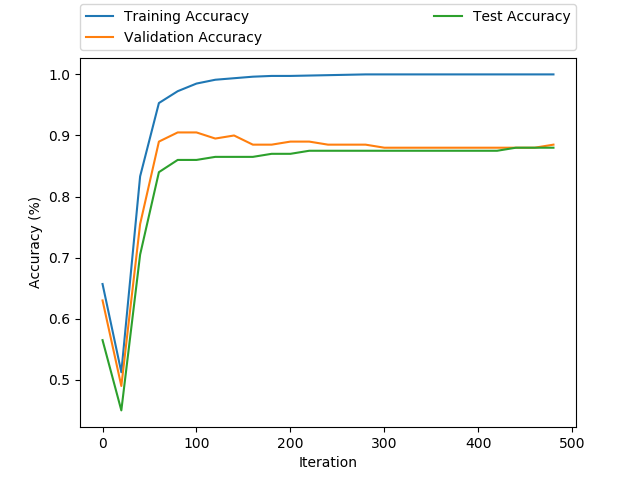
\includegraphics[width=0.8\textwidth]{part4_iteration_vs_accuracy.png}
\end{figure}

\clearpage

\begin{homeworkProblem}
For Logistic Regression, in Part $4$ we showed that the vectorized softmax output for either class is:

$$ = \begin{bmatrix}
\frac{1}{ 1  + \exp( (\theta^{(2)}-\theta^{(1)})^\top x ) }
\\
1 - \frac{1}{ 1  + \exp( (\theta^{(2)}-\theta^{(1)})^\top x ) }
\end{bmatrix}$$

Just as in binary logistic regression, we choose the class with the $argmax$ probability. This is the same as choosing $y=1$ if $$\frac{1}{ 1  + \exp( (\theta^{(2)}-\theta^{(1)})^\top x ) } > 0.5 \iff (\theta^{(2)}-\theta^{(1)})x > 0$$.

Previously, we assumed that the bias term was included in the $\theta$'s. Now we can bring it out:

$$(\theta^{(2)}-\theta^{(1)})x + (b^{(2)} - b^{(1)}) > 0$$

$$ = (b^{(2)} - b^{(1)}) + (\theta^{(2)}_{1}-\theta^{(1)}_{1})x_{1} + (\theta^{(2)}_{2}-\theta^{(1)}_{2})x_{2} + \ldots + (\theta^{(2)}_{k}-\theta^{(1)}_{k})x_{k} > 0$$

Thus for the expression $\theta_{0} + \theta_{1}I_{1}(x) + \theta_{2}I_{2}(x) + \ldots + \theta_{k}I_{k}(x) > thr$, each $I_{i}(x)$ represents the presence of the word $a_{i}$ from the vocabulary in the sample review $x$ (value is 0 or 1). $k$ is the size of the vocabulary (the total number of unique words in the training set from both the positive and negative classes). $\theta_{0}$ represents the difference in the bias of the units $(b^{(2)} - b^{(1)})$. The coefficient $\theta_{i}$ of each $I_{i}(x)$ corresponds to $(\theta^{(2)}_{i}-\theta^{(1)}_{i})$ in the expression above, which is the weight connecting the output unit for the negative class $(1)$ to the input unit $x_{i}$ subtracted from the weight connecting the output unit for the positive class $(2)$ to the input unit $x_{i}$. Thus $\theta_{i}$ represents the polarity of the $i^{th}$ keyword. If the $i^{th}$ keyword is strongly positive, $\theta_{i}$ is strongly positive, and vice-versa.\\\\

For Naive Bayes, when we classify a sample review, we choose the $argmax$ of the conditional probabilities of each class ($1=positive$ or $0=negative$) conditioned on the sample review. This is the same as choosing $y=1$ if
$$\frac{P(class=1 | a_{1},\ldots,a_{n})}{P(class=0 | a_{1},\ldots,a_{n})} > 1$$

If we apply a log to either side of the inequality we have

$$\log(P(class=1 | a_{1},\ldots,a_{n})) - \log(P(class=0 | a_{1},\ldots,a_{n})) > 0$$

Expanding out we have

$\sum_i\Big(\log(P(a_{i} | class=1))\Big) + \log(P(class=1)) - \log(P(a_{i},\ldots,a_{n}))$\\$
-\sum_i\Big(\log(\frac{(P(a_{i}=1 | class=0))}{count(class=0)})\Big) - \log(P(class=0)) - (- \log(P(a_{i},\ldots,a_{n}))) > 0$

$$ = \log\Big(\frac{P(class=1)}{P(class=0)}\Big) + \sum_i\Big(\log(P(a_{i} | class=1)) - \log(P(a_{i} | class=0))\Big) > 0$$

Thus if the expression $\theta_{0} + \theta_{1}I_{1}(x) + \theta_{2}I_{2}(x) + \ldots + \theta_{k}I_{k}(x) > thr$ represents the classification of a single sample review, the bias term $\theta_{0}$ is the log of the ratio of prior probability of the positive class to the negative class. $k$ is the size of the vocabulary (the total number of unique words in the training set from both the positive and negative classes). Each $I_{i}$ is a binary $0$ or $1$ value representing the presence of the $i^{th}$ keyword from the vocabulary in the sample review. The corresponding coefficient $\theta_{i}$ is the log odds value for the word $a_{i}$ we obtained in Part $3$. $\theta_{i}$. $\theta_{i}$ should represent the polarity value of the $i^{th}$ word. As explained in Part 3, the log odds value for the word represents the bias of one label versus another.


\end{homeworkProblem}

\clearpage

\begin{homeworkProblem}
Each $\theta_{i}$ corresponds to the polarity value of the $i^{th}$ word in the training set vocabulary, as explained in Part 6. We are choosing the 100 greatest (most positive) $\theta$s, which means we are selecting the $\theta$s of the words with the strongest polarity for the positive class of reviews. \\

From the results we can see that Naive bayes and Logistic regression select some of the same words in their top 100. Examples include 'outstanding', 'terrific', and 'wonderfully', which qualitatively are very positive. Among both there exist noisy words such as 'also' with a ranking of 3 for logistic regression, and 'gattaca' with a ranking of 5 for Naive Bayes. Some of these may be explained by the bias in the training data since positive reviews are longer than negative reviews, thus there is a chance that a word such as 'also' may appear in more positive reviews. \\

It appears that Naive Bayes more consistently selects keywords with a more immediately strong positive emotion in its top 100 than Logistic regression, for example 'uplifting', 'melancholy', 'lovingly', and 'masterfully' are selected by Naive Bayes but are not present in the list for Logistic Regression. There are more adjectives and adverbs for Naive Bayes. In Logistic Regression in the top of the list we can immediately see words that are not as descriptive; some are nouns, some can be used as emphasis or complimenting words for a positive description. For example, 'life', 'most', 'especially', 'true', 'both', 'together', 'many' are words that are unique to the top 100 for Logistic Regression. These patterns can perhaps be explained by the differences in the models. \\

In Naive Bayes, each feature's weight is set independently, based on how much it correlates with the label. The result is that that if some of the features are dependent on each other and they often occur together (especially if the feature space is large), the prediction might be overestimating their influence in the whole sample space because we are multiplying probability values of two or more highly correlated features that really represent a single feature, and assume that these features could encapsulate a large union of positive training samples, whereas in reality they cover a smaller intersection. Thus, we see many similar adjectives and adverbs selected and pairings such as ('masterfully' and 'weaves'), which may occur together in the text, for the many of the same texts, but are not necessarily the most representative of the entire sample space. For instance, it may not always be the case that the review would contain 'masterfully' or 'weaves'. However, in logistic regression, all the weights are set together such that the linear decision function tends to be high for positive classes and low for negative classes. Thus Logistic Regression may relax the Naive Bayes assumption and be able to compensate for correlated features by weighting them lower. In fact, we see words that are more peculiar as a positive description, but may be even more generalized than Naive Bayes. For example, 'life' and 'fun'. \\

Finally, the theta values for logistic regression are smaller than for Naive Bayes. This is could be due again to the fact that NB fits feature weights independently, while LR accounts for correlations amongst features and thus together with regularization sets weights to be smaller.

\begin{verbatim}
================== RUNNING PART 6 ===================
Printing top 100 thetas for logistic regression: 

Theta 1 0.370288282633 Pos Word: hilarious
Theta 2 0.341819703579 Pos Word: others
Theta 3 0.32956302166 Pos Word: also
Theta 4 0.310441970825 Pos Word: fun
Theta 5 0.29780715704 Pos Word: life
Theta 6 0.295863032341 Pos Word: perfectly
Theta 7 0.293822616339 Pos Word: memorable
Theta 8 0.292977154255 Pos Word: most
Theta 9 0.286952733994 Pos Word: terrific
Theta 10 0.281670749187 Pos Word: overall
Theta 11 0.281082808971 Pos Word: performances
Theta 12 0.276417016983 Pos Word: sometimes
Theta 13 0.264105260372 Pos Word: american
Theta 14 0.263832807541 Pos Word: perfect
Theta 15 0.259931981564 Pos Word: especially
Theta 16 0.256685435772 Pos Word: well
Theta 17 0.254457831383 Pos Word: true
Theta 18 0.254110217094 Pos Word: job
Theta 19 0.249710828066 Pos Word: both
Theta 20 0.249392807484 Pos Word: together
Theta 21 0.247464090586 Pos Word: yet
Theta 22 0.244372099638 Pos Word: quite
Theta 23 0.243289008737 Pos Word: wonderfully
Theta 24 0.238423168659 Pos Word: many
Theta 25 0.238133817911 Pos Word: very
Theta 26 0.237949088216 Pos Word: excellent
Theta 27 0.236174911261 Pos Word: performance
Theta 28 0.235593289137 Pos Word: enjoyable
Theta 29 0.229307442904 Pos Word: seen
Theta 30 0.228570848703 Pos Word: best
Theta 31 0.228331148624 Pos Word: great
Theta 32 0.223626852036 Pos Word: makes
Theta 33 0.220908969641 Pos Word: details
Theta 34 0.219353586435 Pos Word: different
Theta 35 0.217106878757 Pos Word: flaws
Theta 36 0.210115492344 Pos Word: ending
Theta 37 0.207596465945 Pos Word: people
Theta 38 0.206161439419 Pos Word: family
Theta 39 0.205819502473 Pos Word: light
Theta 40 0.205211788416 Pos Word: deserves
Theta 41 0.203720211983 Pos Word: your
Theta 42 0.20241111517 Pos Word: world
Theta 43 0.200672328472 Pos Word: though
Theta 44 0.200606048107 Pos Word: pace
Theta 45 0.200246855617 Pos Word: set
Theta 46 0.19957524538 Pos Word: simple
Theta 47 0.198278710246 Pos Word: ive
Theta 48 0.197140872478 Pos Word: while
Theta 49 0.197102129459 Pos Word: brilliant
Theta 50 0.196320056915 Pos Word: works
Theta 51 0.195221245289 Pos Word: easily
Theta 52 0.194099128246 Pos Word: him
Theta 53 0.193452358246 Pos Word: town
Theta 54 0.193373888731 Pos Word: chemistry
Theta 55 0.192798674107 Pos Word: throughout
Theta 56 0.192309722304 Pos Word: extremely
Theta 57 0.190947294235 Pos Word: gives
Theta 58 0.18970644474 Pos Word: definitely
Theta 59 0.189220011234 Pos Word: fight
Theta 60 0.187702104449 Pos Word: although
Theta 61 0.18651214242 Pos Word: four
Theta 62 0.18610650301 Pos Word: may
Theta 63 0.184525519609 Pos Word: soundtrack
Theta 64 0.184228926897 Pos Word: right
Theta 65 0.182777166367 Pos Word: see
Theta 66 0.18255341053 Pos Word: allows
Theta 67 0.181220784783 Pos Word: twists
Theta 68 0.179337233305 Pos Word: portrayed
Theta 69 0.178353592753 Pos Word: outstanding
Theta 70 0.178338199854 Pos Word: enjoyed
Theta 71 0.173395931721 Pos Word: surprised
Theta 72 0.171155959368 Pos Word: wonderful
Theta 73 0.171056509018 Pos Word: naturally
Theta 74 0.169605761766 Pos Word: entertaining
Theta 75 0.169468715787 Pos Word: change
Theta 76 0.16915653646 Pos Word: class
Theta 77 0.167777106166 Pos Word: today
Theta 78 0.167124301195 Pos Word: back
Theta 79 0.167083710432 Pos Word: era
Theta 80 0.167033970356 Pos Word: leave
Theta 81 0.165266931057 Pos Word: oscar
Theta 82 0.165243148804 Pos Word: realistic
Theta 83 0.164840936661 Pos Word: intelligent
Theta 84 0.164191395044 Pos Word: above
Theta 85 0.162372589111 Pos Word: pulp
Theta 86 0.162127256393 Pos Word: subtle
Theta 87 0.162071466446 Pos Word: bill
Theta 88 0.161928340793 Pos Word: couple
Theta 89 0.161036044359 Pos Word: takes
Theta 90 0.160862445831 Pos Word: eventually
Theta 91 0.159853026271 Pos Word: classic
Theta 92 0.159403383732 Pos Word: thankfully
Theta 93 0.159205660224 Pos Word: other
Theta 94 0.158646672964 Pos Word: breathtaking
Theta 95 0.157781720161 Pos Word: follows
Theta 96 0.157499045134 Pos Word: plenty
Theta 97 0.156933516264 Pos Word: break
Theta 98 0.156833425164 Pos Word: shows
Theta 99 0.156503647566 Pos Word: still
Theta 100 0.15550801158 Pos Word: mind


Printing top 100 thetas for naive bayes: 

Theta 1 2.13585539483 Pos Word: outstanding
Theta 2 2.03676449218 Pos Word: astounding
Theta 3 1.90323309956 Pos Word: fashioned
Theta 4 1.90323309956 Pos Word: dread
Theta 5 1.88521459406 Pos Word: wonderfully
Theta 6 1.8291251274 Pos Word: gattaca
Theta 7 1.74908241973 Pos Word: lovingly
Theta 8 1.74908241973 Pos Word: ideals
Theta 9 1.69192400589 Pos Word: spielbergs
Theta 10 1.69192400589 Pos Word: bold
Theta 11 1.68008954824 Pos Word: flawless
Theta 12 1.68008954824 Pos Word: damon
Theta 13 1.66207104274 Pos Word: weaknesses
Theta 14 1.66207104274 Pos Word: weakness
Theta 15 1.66207104274 Pos Word: offbeat
Theta 16 1.66207104274 Pos Word: notoriety
Theta 17 1.66207104274 Pos Word: niccol
Theta 18 1.66207104274 Pos Word: masterfully
Theta 19 1.66207104274 Pos Word: en
Theta 20 1.66207104274 Pos Word: downside
Theta 21 1.66207104274 Pos Word: continuing
Theta 22 1.66207104274 Pos Word: coens
Theta 23 1.66207104274 Pos Word: burbank
Theta 24 1.63129938407 Pos Word: hatred
Theta 25 1.63129938407 Pos Word: avoids
Theta 26 1.62233071409 Pos Word: finest
Theta 27 1.61555102711 Pos Word: era
Theta 28 1.59955068576 Pos Word: anger
Theta 29 1.56676086294 Pos Word: mixing
Theta 30 1.56676086294 Pos Word: uplifting
Theta 31 1.56676086294 Pos Word: uncut
Theta 32 1.56676086294 Pos Word: trumans
Theta 33 1.56676086294 Pos Word: melancholy
Theta 34 1.56676086294 Pos Word: marvelous
Theta 35 1.56676086294 Pos Word: jude
Theta 36 1.56676086294 Pos Word: introspective
Theta 37 1.56676086294 Pos Word: freed
Theta 38 1.56676086294 Pos Word: crimson
Theta 39 1.56676086294 Pos Word: brisk
Theta 40 1.52593886842 Pos Word: religion
Theta 41 1.52593886842 Pos Word: poignant
Theta 42 1.52593886842 Pos Word: magnificent
Theta 43 1.51546756855 Pos Word: chilling
Theta 44 1.49776799145 Pos Word: thematic
Theta 45 1.49776799145 Pos Word: strengths
Theta 46 1.47714870425 Pos Word: beautifully
Theta 47 1.46140034728 Pos Word: weaves
Theta 48 1.46140034728 Pos Word: unassuming
Theta 49 1.46140034728 Pos Word: topping
Theta 50 1.46140034728 Pos Word: tool
Theta 51 1.46140034728 Pos Word: sparked
Theta 52 1.46140034728 Pos Word: soviet
Theta 53 1.46140034728 Pos Word: skarsgard
Theta 54 1.46140034728 Pos Word: separately
Theta 55 1.46140034728 Pos Word: rebels
Theta 56 1.46140034728 Pos Word: outlook
Theta 57 1.46140034728 Pos Word: noah
Theta 58 1.46140034728 Pos Word: mustsee
Theta 59 1.46140034728 Pos Word: meryl
Theta 60 1.46140034728 Pos Word: linney
Theta 61 1.46140034728 Pos Word: layered
Theta 62 1.46140034728 Pos Word: jordans
Theta 63 1.46140034728 Pos Word: jo
Theta 64 1.46140034728 Pos Word: jabba
Theta 65 1.46140034728 Pos Word: hypocrisy
Theta 66 1.46140034728 Pos Word: hesitation
Theta 67 1.46140034728 Pos Word: hawthorne
Theta 68 1.46140034728 Pos Word: gunplay
Theta 69 1.46140034728 Pos Word: gretchen
Theta 70 1.46140034728 Pos Word: flynt
Theta 71 1.46140034728 Pos Word: existed
Theta 72 1.46140034728 Pos Word: envy
Theta 73 1.46140034728 Pos Word: drawback
Theta 74 1.46140034728 Pos Word: divine
Theta 75 1.46140034728 Pos Word: devilish
Theta 76 1.46140034728 Pos Word: carver
Theta 77 1.46140034728 Pos Word: aladdin
Theta 78 1.46140034728 Pos Word: performed
Theta 79 1.44540000593 Pos Word: terrific
Theta 80 1.4236600193 Pos Word: spike
Theta 81 1.4236600193 Pos Word: seamless
Theta 82 1.4236600193 Pos Word: reminder
Theta 83 1.4236600193 Pos Word: recalls
Theta 84 1.4236600193 Pos Word: mulan
Theta 85 1.4236600193 Pos Word: missteps
Theta 86 1.4236600193 Pos Word: keen
Theta 87 1.4236600193 Pos Word: fascination
Theta 88 1.4236600193 Pos Word: elliot
Theta 89 1.4236600193 Pos Word: detract
Theta 90 1.4236600193 Pos Word: deft
Theta 91 1.4236600193 Pos Word: cheerful
Theta 92 1.4236600193 Pos Word: captures
Theta 93 1.4236600193 Pos Word: addresses
Theta 94 1.40424193344 Pos Word: regard
Theta 95 1.40424193344 Pos Word: gripping
Theta 96 1.40424193344 Pos Word: depicted
Theta 97 1.40424193344 Pos Word: innocence
Theta 98 1.37438897029 Pos Word: refreshing
Theta 99 1.37438897029 Pos Word: breathtaking
Theta 100 1.34361731162 Pos Word: workings
\end{verbatim}

\end{homeworkProblem}

\clearpage


\end{homeworkProblem}
\clearpage








%----------------------------------------------------------------------------------------

\end{document}